\documentclass[preprint2]{aastex631}
\received{\today}
\shorttitle{Improved NEO Classification}
\graphicspath{{figures/}}

\usepackage{lipsum}
\usepackage{physics}
\usepackage{multirow}
\usepackage{xspace}
\usepackage{natbib}
\usepackage{fontawesome5}
\usepackage{xcolor}
\usepackage{wrapfig}
\usepackage[figuresright]{rotating}

% remove indents in footnotes
\usepackage[hang,flushmargin]{footmisc} 

\newcommand{\todo}[1]{{\color{red}{[TODO: #1}]}}
\newcommand{\needcite}{{\color{magenta}{(needs citation)}}}
\newcommand{\placeholder}[1]{{\color{gray} \lipsum[#1]}}

% custom function for adding units
\makeatletter
\newcommand{\unit}[1]{%
    \,\mathrm{#1}\checknextarg}
\newcommand{\checknextarg}{\@ifnextchar\bgroup{\gobblenextarg}{}}
\newcommand{\gobblenextarg}[1]{\,\mathrm{#1}\@ifnextchar\bgroup{\gobblenextarg}{}}
\makeatother

\newcommand{\dig}{\texttt{digest2}}
\newcommand{\sss}{S3M}
\newcommand{\mpco}{MPCORB}

\begin{document}

\title{{\large An improved classification scheme for distinguishing NEOs from MBAs}\\\vspace{0.15cm}ASTR 597A Final Project}

% affiliations
\newcommand{\UW}{Department of Astronomy, University of Washington, Seattle, WA, 98195}

\author[0000-0001-6147-5761]{Tom Wagg}
\affiliation{\UW}

\correspondingauthor{Tom Wagg}
\email{tomwagg@uw.edu}

% \begin{abstract}
%     todo
% \end{abstract}

\keywords{}

\section{Introduction}

\begin{itemize}
    \item Explain why were care about NEOs
    \item Point out that LSST is going to make detections explode
    \item Highlight that \dig{} \citep{Keys+2019} isn't ready for the MBA background (Fig.~\ref{fig:digest2_should_be_scared})
    \item Explain how using more than simple orbital parameters could improve matters
\end{itemize}

\begin{figure}[htb]
    \centering
    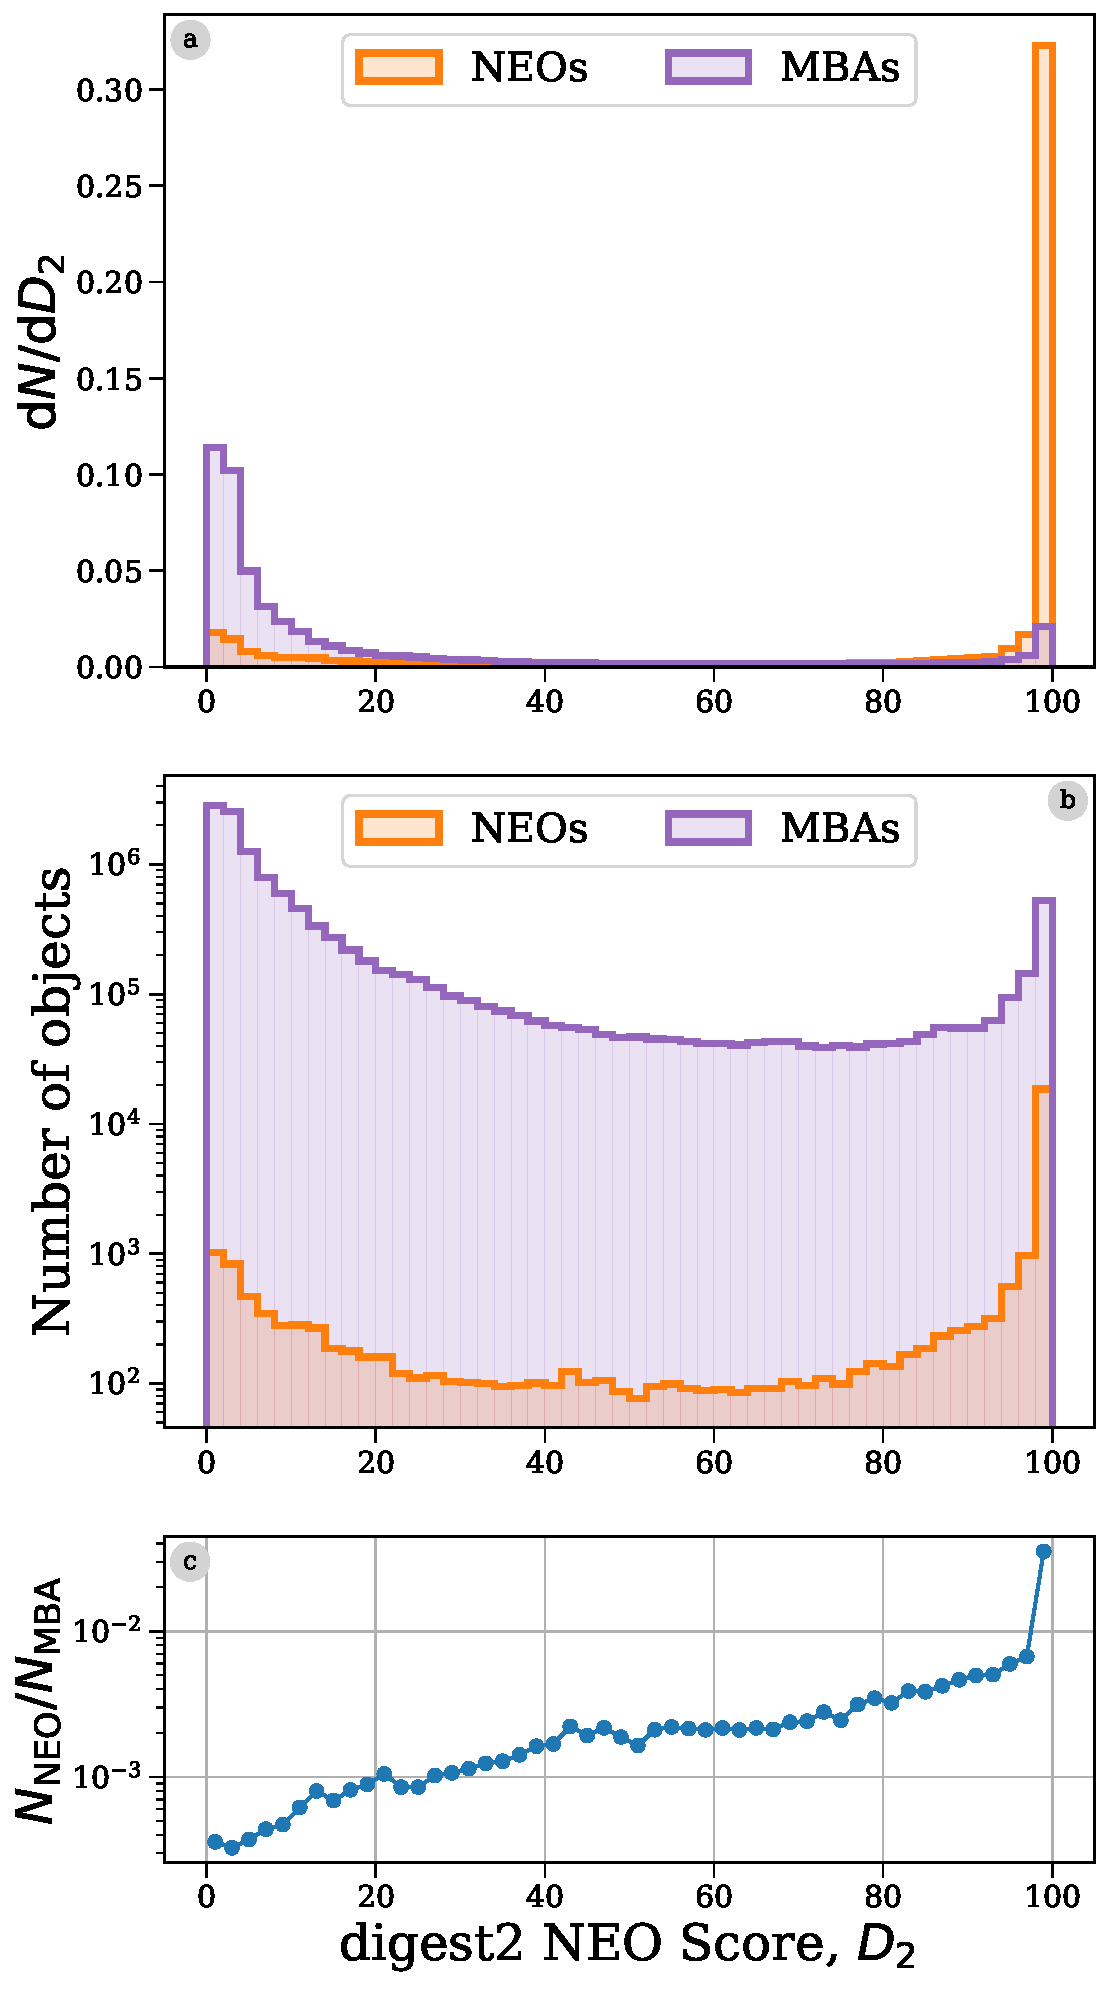
\includegraphics[width=\columnwidth]{digest2_pollution.pdf}
    \caption{\dig{} scores for all NEOs and MBAs observed in the first year of our simulated LSST observations. \textbf{(a)} normalised histograms of \dig{} scores, \textbf{(b)} the same histograms un-normalised \textbf{(c)} ratio of the histograms in (b). Note that the latter two panels are on a logarithmic scale.}
    \label{fig:digest2_should_be_scared}
\end{figure}

\section{Methods}

\begin{itemize}
    \item MBAs are constrained to lie in the ecliptic plane - we can leverage this
    \item Tracklet selection conditions
    \item Ecliptic latitude split the population well directly because of this
    \item Direction of motion relative to the ecliptic plane works too since closer things aren't constrained as strongly
    \item Show plots of both of them
\end{itemize}

\section{Results}

\begin{itemize}
    \item Combine all 3 into 1 score, plot that up, compare to earlier one
    \item Decide on threshold and analyse performance with contingency matrix
    \item (Consider whether we could weight the different parameters differently to improve matters)
\end{itemize}

\section{Discussion}

\begin{itemize}
    \item Recommend sorting rather than just a threshold
    \item Coordination between groups will be important NEOFixer
\end{itemize}

\section{Conclusion}

\begin{itemize}
    \item Point out whether we did better :shrug:
\end{itemize}

\bibliographystyle{aasjournal}
\bibliography{refs}{}

\end{document}